\documentclass{article}
\usepackage{fullpage}
\usepackage{multicol,multirow}
\usepackage{tabularx}
\usepackage{ulem}
\usepackage[utf8]{inputenc}
\usepackage[russian]{babel}
\usepackage{pgfplots}
\usepackage{graphicx}

\begin{document}

\section*{Лабораторная работа №6 по курсу «Численные методы»}

Выполнил студент группы М8О-408Б-20 Блинов Максим.
\\
Преподаватель: Пивоваров Д.\,Е.

\subsection*{Цель}

Используя явную схему крест и неявную схему, решить начально-краевую задачу 
для дифференциального уравнения гиперболического типа. Осуществить реализацию 
трех вариантов аппроксимации граничных условий, содержащих производные: 
двухточечная аппроксимация с первым порядком, трехточечная аппроксимация со вторым порядком, 
двухточечная аппроксимация со вторым порядком. В различные моменты времени вычислить 
погрешность численного решения путем сравнения результатов с приведенным в задании аналитическим решением U(x, t).

\subsection*{Вариант 3}
$$\frac{\partial^2 u}{\partial t^2} = \frac{\partial^2 u}{\partial x^2} - 3u,$$
$$u(0, t) = \sin(2t),$$
$$u(\pi, t) = - \sin(2t),$$
$$u(x, 0) = 0,$$
$$u_t(x, 0) = 2 \cos x.$$
\text{Аналитическое решение: } $$U(x, t) = \cos x \sin(2t).$$



\subsection*{О программе}

Программа была реализована на языке программирования Go и включает в себя три численных метода для решения дифференциальных уравнений: 
явный метод (explicit), неявный метод (implicit) и метод Кранка-Николсона (Crank-Nicolson). Для визуализации результатов использовалась библиотека Gonum, 
которая предоставляет широкие возможности для построения графиков в среде Go. Результаты вычислений иллюстрируют поведение решений в зависимости от времени 
и начальных условий, а также позволяют оценить точность численных методов путём сравнения с аналитическим решением задачи. 
Графики ошибок демонстрируют различия между аналитическими и численными решениями на протяжении всего временного интервала. 
Все вычислительные эксперименты и генерация графиков проводились в рамках данной программы.

\subsection*{Инструкция к запуску}
Для запуска программы на Go, решающей гиперболические дифференциальные уравнения, убедитесь, что у вас установлена последняя версия Go 
(на данный момент 1.21, проверьте на официальном сайте). Создайте рабочее пространство, затем установите необходимые зависимости go mod tidy.

\pagebreak

\subsection*{Явная конечно-разностная схема}

В исходном уравнении перейдем от производных к их численным приближениям. Вторую производную будем аппроксимировать
по значениям нижнего временного слоя.

Получим рекуррентное соотношение:
\[
u_{j}^{k+1} = \sigma \left( u_{j+1}^{k} - 2u_{j}^{k} + u_{j-1}^{k} \right) + \left( 2 - 3\tau^2 \right)u_{j}^{k} - u_{j}^{k-1}
\]
где \(\sigma = \frac{\tau^2}{h^2}\).

Для нижнего временного ряда:
\[
u_{j}^{0} = \psi_1(x_j)
\]
\[
u_{j}^{1} = \psi_1(x_j) + \psi_2(x_j)\tau
\]

Остальные значения \( u \) в нижнем временном ряду известны из начальных условий. Далее можем в цикле проходиться по сетке и
рекуррентно считать значения в ней по полученной формуле.

\textit{Примечание:} можно было повысить порядок аппроксимации для \( u_{j}^{1} \), но т.к. в моем случае \(\psi_1 = 0\), то и вторая производная
от нее будет равна нулю, а следовательно повышение порядка бессмысленно.


\subsection*{Неявная конечно-разностная схема}

В исходном уравнении перейдем от производных к их численным приближениям. Вторую производную будем аппроксимировать
по значениям верхнего временного слоя.

Чтобы получить значения \( u \) в одном временном ряду, необходимо решить систему уравнений:
\[
\begin{cases}
b_1u_{j}^{k+1} + c_1u_{j+1}^{k+1} = d_1, & j = 1, \\
a_ju_{j-1}^{k+1} + b_ju_{j}^{k+1} + c_ju_{j+1}^{k+1} = d_j, & j = 2 \ldots N - 2, \\
a_{N-1}u_{N-2}^{k+1} + b_{N-1}u_{N-1}^{k+1} = d_{N-1}, & j = N - 1.
\end{cases}
\]
где
\[
a_j = c_j = \sigma
\]
\[
b_j = -(1 + 2\sigma + 3\tau^2)
\]
\[
d_j = -2u_{j}^{k} + u_{j}^{k-1}, \quad j = 2 \ldots N - 2
\]
\[
d_1 = -(u_{1}^{k} + \sigma \phi(t^{k+1}))
\]
\[
d_{N-1} = -(u_{N-1}^{k} + \sigma \phi(t^{k+1}))
\]

\pagebreak
\subsection*{Результаты}
\begin{center}
Полученные вычисления на момент времени $ t = 0.5 $
\\
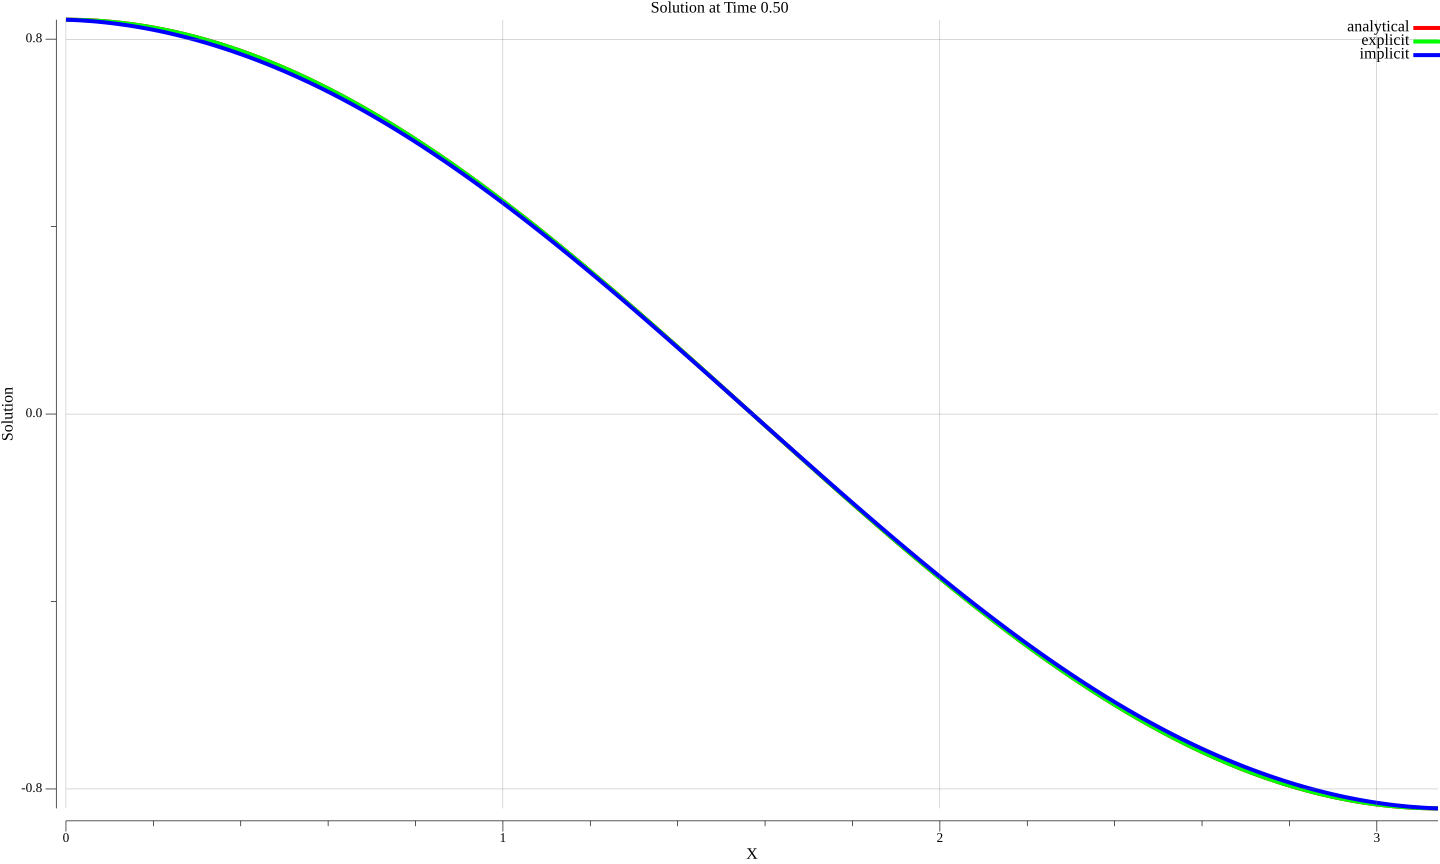
\includegraphics[scale=0.3]{solutions.png}
\\


Изменение погрешности
\\
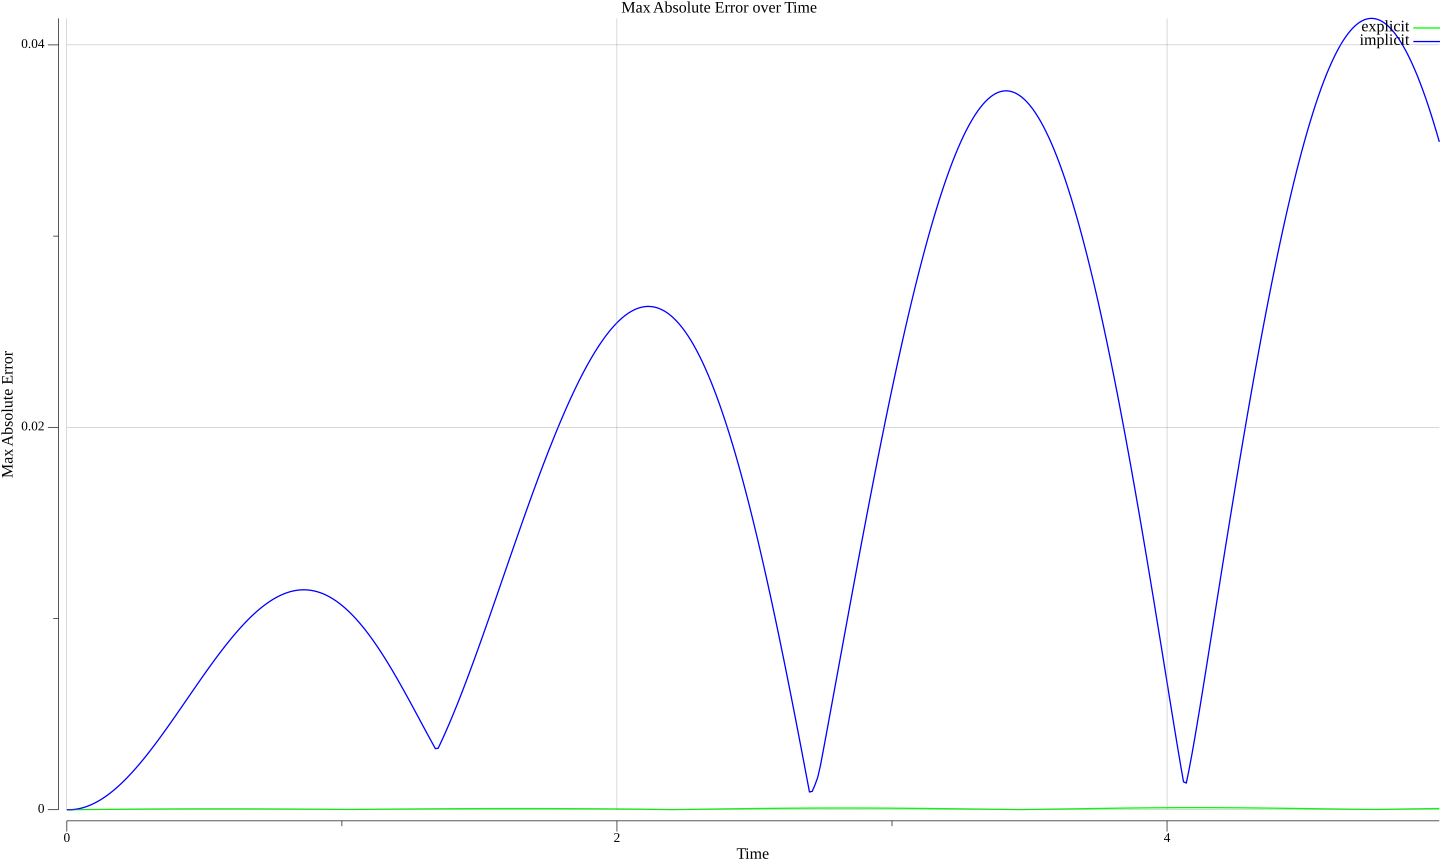
\includegraphics[scale=0.3]{error_plot1.png}

\pagebreak
explicit
\\
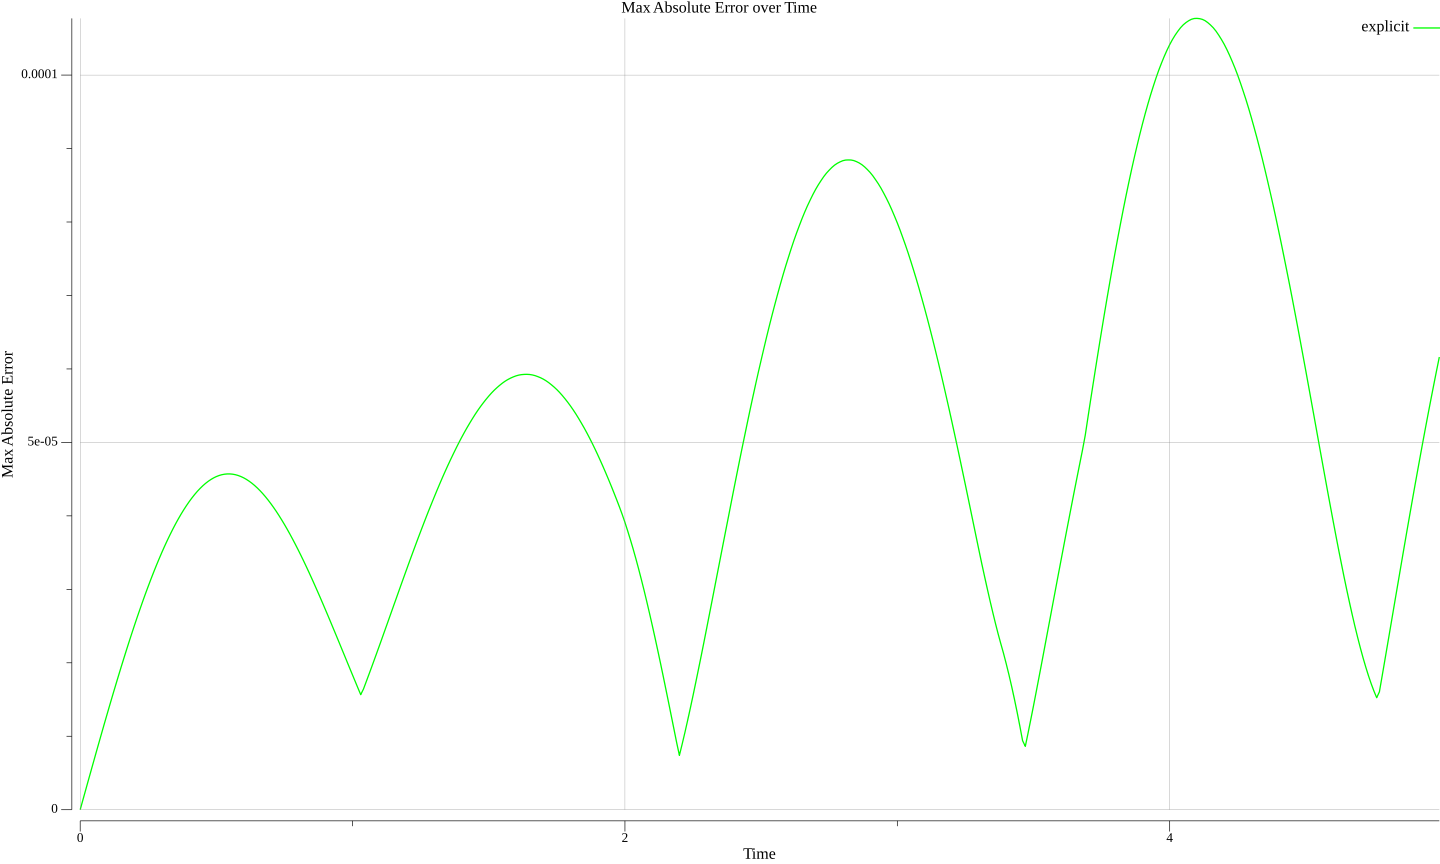
\includegraphics[scale=0.3]{error_plot2.png}
\end{center}

\subsection*{Вывод программы}
\\
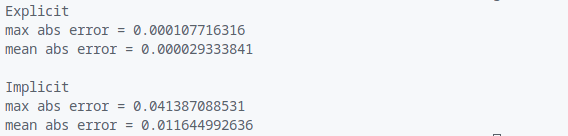
\includegraphics[scale=0.7]{console.png}
\\

\subsection*{Вывод}

В ходе выполнения данной работы мной были освоены методы решения начально-краевых задач для гиперболических дифференциальных уравнений, а именно:

- Использование явной конечно-разностной схемы.

- Применение неявной конечно-разностной схемы.
Оба метода позволили достичь адекватной точности в решении поставленной задачи.

Отмечу, что явная схема отличается простотой вычислений, однако ее применимость ограничена условной устойчивостью и требует аккуратного подбора параметров сетки для получения достоверного результата.

В то же время, неявная схема требует более глубоких вычислений, но обеспечивает абсолютную устойчивость, что делает ее предпочтительной для широкого диапазона параметров.
\end{document}